%%
%% Copyright 2007, 2008, 2009 Elsevier Ltd
%%
%% This file is part of the 'Elsarticle Bundle'.
%% ---------------------------------------------
%%
%% It may be distributed under the conditions of the LaTeX Project Public
%% License, either version 1.2 of this license or (at your option) any
%% later version.  The latest version of this license is in
%%    http://www.latex-project.org/lppl.txt
%% and version 1.2 or later is part of all distributions of LaTeX
%% version 1999/12/01 or later.
%%
%% The list of all files belonging to the 'Elsarticle Bundle' is
%% given in the file `manifest.txt'.
%%

%% Template article for Elsevier's document class `elsarticle'
%% with numbered style bibliographic references
%% SP 2008/03/01

\documentclass[preprint,12pt,a4paper]{elsarticle}

%% Use the option review to obtain double line spacing
%% \documentclass[authoryear,preprint,review,12pt]{elsarticle}

%% For including figures, graphicx.sty has been loaded in
%% elsarticle.cls. If you prefer to use the old commands
%% please give \usepackage{epsfig}

%% The amssymb package provides various useful mathematical symbols
\usepackage{amssymb}
%% The amsthm package provides extended theorem environments
%% \usepackage{amsthm}

%% The lineno packages adds line numbers. Start line numbering with
%% \begin{linenumbers}, end it with \end{linenumbers}. Or switch it on
%% for the whole article with \linenumbers.
\usepackage{lineno}

\usepackage{float}
\restylefloat{table}

% ======== additional package not in SoftwareX template ========
\usepackage[colorlinks=true, urlcolor=blue, pdfborder={0 0 0}]{hyperref}
\usepackage{breakurl}
\usepackage[htt]{hyphenat}
%\usepackage{listings}
\usepackage{xcolor}
%\usepackage{todonotes}

% \let\oldtodo\todo
% \renewcommand{\todo}[1]{\oldtodo[tickmarkheight=0.5em]{#1}}

\newcommand{\comment}[1]{}
% =================================================

\journal{SoftwareX}

\begin{document}
\begin{frontmatter}

\title{\texttt{davos}: a Python package ``smuggler'' for constructing
  lightweight reproducible notebooks}
\author{Paxton C. Fitzpatrick}
\author{Jeremy R. Manning\corref{cor}}
\ead{Jeremy.R.Manning@Dartmouth.edu}
\cortext[cor]{Corresponding author}
\address{Department of Psychological and Brain Sciences\\Dartmouth College, Hanover, NH 03755}

% ------------------------------------------------------ ABSTRACT ------------------------------------------------------

\begin{abstract}
% 100-word limit (though many published articles don't seem to conform
% to this?)

  Reproducibility is a core requirement of modern scientific research.
  For computational research, reproducibility means that code should
  produce the same results, even when run on different systems.  A
  standard approach to ensuring reproducibility entails packaging a
  project's dependencies along with its primary code base.  Existing
  solutions vary in how deeply these dependencies are specified,
  ranging from virtual environments, to containers, to virtual
  machines.  Each of these existing solutions requires installing or
  setting up a system for running the desired code, increasing the
  complexity and time cost of sharing or engaging with reproducible
  science. Here, we propose a lighter-weight solution:  the
  \texttt{davos} library.  When used in combination with a
  notebook-based Python project, \texttt{davos} provides a
  mechanism for specifying (and automatically installing) the correct
  versions of the project's dependencies.  The \texttt{davos}
  library further ensures that those packages and specific versions are used every time the
  notebook's code is executed.  This enables researchers to share a complete
  reproducible copy of their code within a single Jupyter notebook file.

\end{abstract}


\begin{keyword}
Reproducibility \sep Open science \sep Python \sep Jupyter Notebook \sep Google Colaboratory \sep Package management
\end{keyword}

\end{frontmatter}


% ------------------------------------------------------ METADATA ------------------------------------------------------
\section*{Required Metadata}

\section*{Current code version}


\begin{table}[H]
\begin{tabular}{|l|p{6.5cm}|p{6.5cm}|}
\hline
\textbf{Nr.} & \textbf{Code metadata description} & \textbf{Metadata value} \\
\hline
C1 & Current code version &  v0.1.1 \\
\hline
C2 & Permanent link to code/repository used for this code version & \url{https://github.com/ContextLab/davos/tree/v0.1.1} \\
\hline
C3 & Code Ocean compute capsule & \\
\hline
C4 & Legal Code License & MIT \\
\hline
C5 & Code versioning system used & git \\
\hline
C6 & Software code languages, tools, and services used & Python, JavaScript, PyPI/pip, IPython, Jupyter, Ipykernel, PyZMQ. Additional tools used for tests: pytest, Selenium, Requests, mypy, GitHub Actions \\
\hline
C7 & Compilation requirements, operating environments, and
     dependencies & Dependencies:~Python $\geq 3.6$, packaging, setuptools.~Supported OSes: MacOS, Linux, Unix-like.~Supported IPython environments: Jupyter notebooks, JupyterLab, Google Colaboratory, Binder, IDE-based notebook editors. \\
\hline
C8 & Link to developer documentation/manual & \url{https://github.com/ContextLab/davos\#readme} \\
\hline
C9 & Support email for questions & contextualdynamics@gmail.com \\
\hline
\end{tabular}
\caption{Code metadata}
\label{}
\end{table}

\linenumbers


% --------------------------------------------- MOTIVATION & SIGNIFICANCE ----------------------------------------------
\section{Motivation and significance}

The same computer code may not behave identically under different
circumstances.  For example, when code depends on external libraries,
different versions of those libraries may function differently.  Or
when CPU or GPU instruction sets differ across machines, the same
high-level code may be compiled into different machine instructions.
Because executing identical code does not guarantee identical
outcomes, code sharing alone is often insufficient for
enabling researchers to reproduce each other's work, or to collaborate on
projects involving data collection or analysis.

Within the Python~\cite{vanR95} community, external
packages that are published in the most popular
repositories~\cite{Pyth03, cond15} are associated with version numbers
and tags that allow users to guarantee they are installing
exactly the same code across different computing environments \cite{CoghStuf13}.
While it is \textit{possible} to manually install the intended
version of every dependency of a Python script or package, manually
tracking down those dependencies can impose a substantial burden on
the user and create room for mistakes and inconsistencies. Further, when dependency versions
are left unspecified, replicating the original computing environment
becomes difficult or impossible.

\begin{figure}[tp]
\centering
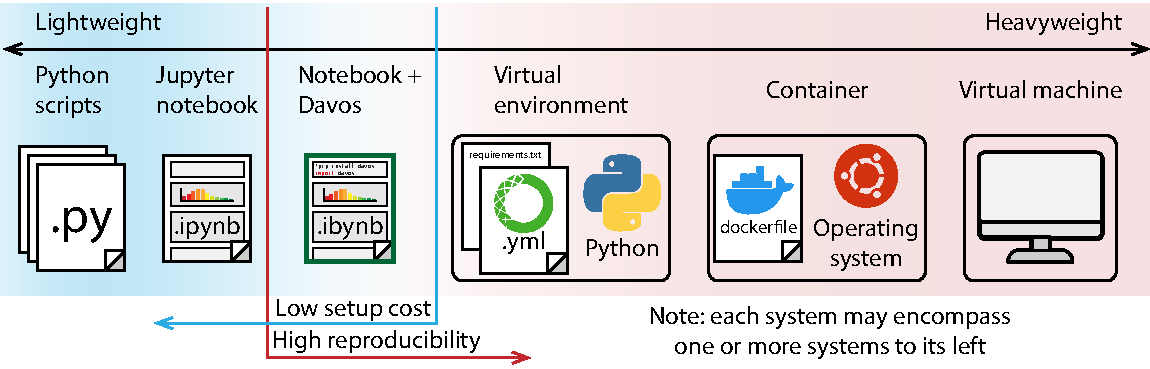
\includegraphics[width=\textwidth]{figs/shareable_code}
\caption{\small \textbf{Systems for sharing code within the Python
    ecosystem.}  From left to right: plain-text \textbf{Python
    scripts} (\texttt{.py} files) provide the most basic ``system''
  for sharing raw code.  Scripts may reference external libraries, but
  those libraries must be manually installed on other users' systems.
  Further, any checking needed to verify that the correct versions of
  those libraries were installed must also be performed manually.
  \textbf{Jupyter notebooks} (\texttt{.ipynb} files) comprise embedded
  text, executable code, and media (including rendered figures, code
  output, etc.).  When the \textbf{\texttt{davos} library} is imported
  into a Jupyter notebook, the notebook's functionality is extended to
  automatically install any required external libraries (at their
  correct versions, when specified).  \textbf{Virtual environments}
  allow users to install an isolated copy of Python and all required
  dependencies. This typically entails distributing a configuration file
  (e.g., a \texttt{pyproject.toml}~\cite{CannEtal16} or \texttt{environment.yml})
  that specifies all project dependencies (including version numbers of
  external libraries) alongside the primary code base. Users can then install
  a third-praty tool~\cite[e.g.,][]{Anac12, Eust19} to read the file and build the environment.
  \textbf{Containers} provide a means of defining an isolated
  environment that includes a complete operating system (independent
  of the user's operating system), in addition to (optionally)
  specifying a virtual environment or other configurations needed to
  provide the necessary computing environment.  Containers are
  typically defined using specification files (e.g., a plain-text
  \texttt{Dockerfile}) that instruct the virtualization engine
  regarding how to build the containerized environment.  \textbf{Virtual
    machines} provide a complete hardware-level simulation of the
  computing environment.  In addition to simulating specific hardware,
  virtual machines (typically specified using binary images files)
  must also define operating system-level properties of the computing
  environment.  Systems to the left of the blue vertical line entail
  sharing individual files, with no additional installation or
  configuration needed to run the target code.  Systems to the right
  of the red vertical line support precise control over dependencies
  and versioning.  Notebooks enhanced using the \texttt{davos} library
  are easily shareable and require minimal setup costs, while also
  facilitating high reproducibility by enabling precise control over
  project dependencies.}
\label{fig:code-sharing}
\end{figure}

Computational researchers and other programmers have developed a broad
set of approaches and tools to facilitate code sharing and
reproducible outcomes (Fig.~\ref{fig:code-sharing}). At one
extreme, simply distributing a set of Python scripts (\texttt{.py} files) may
enable others to use or gain insights into the relevant work. Because
Python is installed by default on most modern operating systems, for
some projects, this may be sufficient. Another popular approach
entails creating Jupyter
notebooks~\cite{KluyEtal16} that comprise a mix of text, executable
code, and embedded media. Notebooks may call or import external
scripts or libraries---even intersperse snippets of other programming
or markup lang\-uages---in order to provide a more compact and readable
experience for users. Both of these systems (Python scripts and
notebooks) provide a convenient means of sharing code, with the
caveat that they do not specify the computing environment in which the
code is executed. Therefore the functionality of code shared using
these systems cannot be guaranteed across different users or setups.

At another extreme, virtual machines~\cite{Gold74, AltiEtal05,
 Rose99} provide a hardware-level simulation of the desired system.
Virtual machines are typically isolated such
that installing or running software on a virtual machine does not
impact the user's primary operating system or computing environment.
Containers~\cite[e.g.,][]{Merk14, KurtEtal17} provide a similar
``isolated'' experience. Although containerized environments do not
specify hardware-level operations, they are typically packaged with a
complete operating system, in addition to a complete copy of Python
and any relevant package dependencies. Virtual
environments~\cite[e.g.,][]{Anac12, Eust19} also provide a computing
environment that is largely separated from the user's main
environment. They incorporate a copy of Python and the target
software's dependencies, but virtual environments do not specify or
reproduce an operating system for the runtime environment. Each of
these systems (virtual machines, containers, and virtual environments)
guarantees (to differing degrees---at the hardware level, operating
system level, and Python environment level, respectively) that the
relevant code will run similarly for different users. However, each
of these systems also relies on additional software that can be
complex or resource-intensive to install and use, creating potential
barriers to both contributing to and taking advantage of open science
resources.

We designed \texttt{davos} to occupy a ``sweet spot'' between these
extremes.  \texttt{davos} is a notebook-installable package that adds
functionality to the default notebook experience. Like standard
Jupyter notebooks, \texttt{davos}-enhanced notebooks allow
researchers to include text, executable code, and media within a
single file. No further setup or installation is required, beyond
what is needed to run standard Jupyter notebooks. And like virtual
environments, \texttt{davos} provides a convenient mechanism for fully
specifying (and installing, as needed) a complete set of Python
dependencies, including package versions.




% ------------------------------------------------ SOFTWARE DESCRIPTION ------------------------------------------------
\section{Software description}
% Describe the software in as much as is necessary to establish a vocabulary needed to explain its impact.
The \texttt{davos} package is named after Davos Seaworth, a smuggler often referred to as ``the Onion Knight" from the series \textit{A Song of Ice and Fire} by George R. R. Martin.

\begin{figure}[tp]
\centering
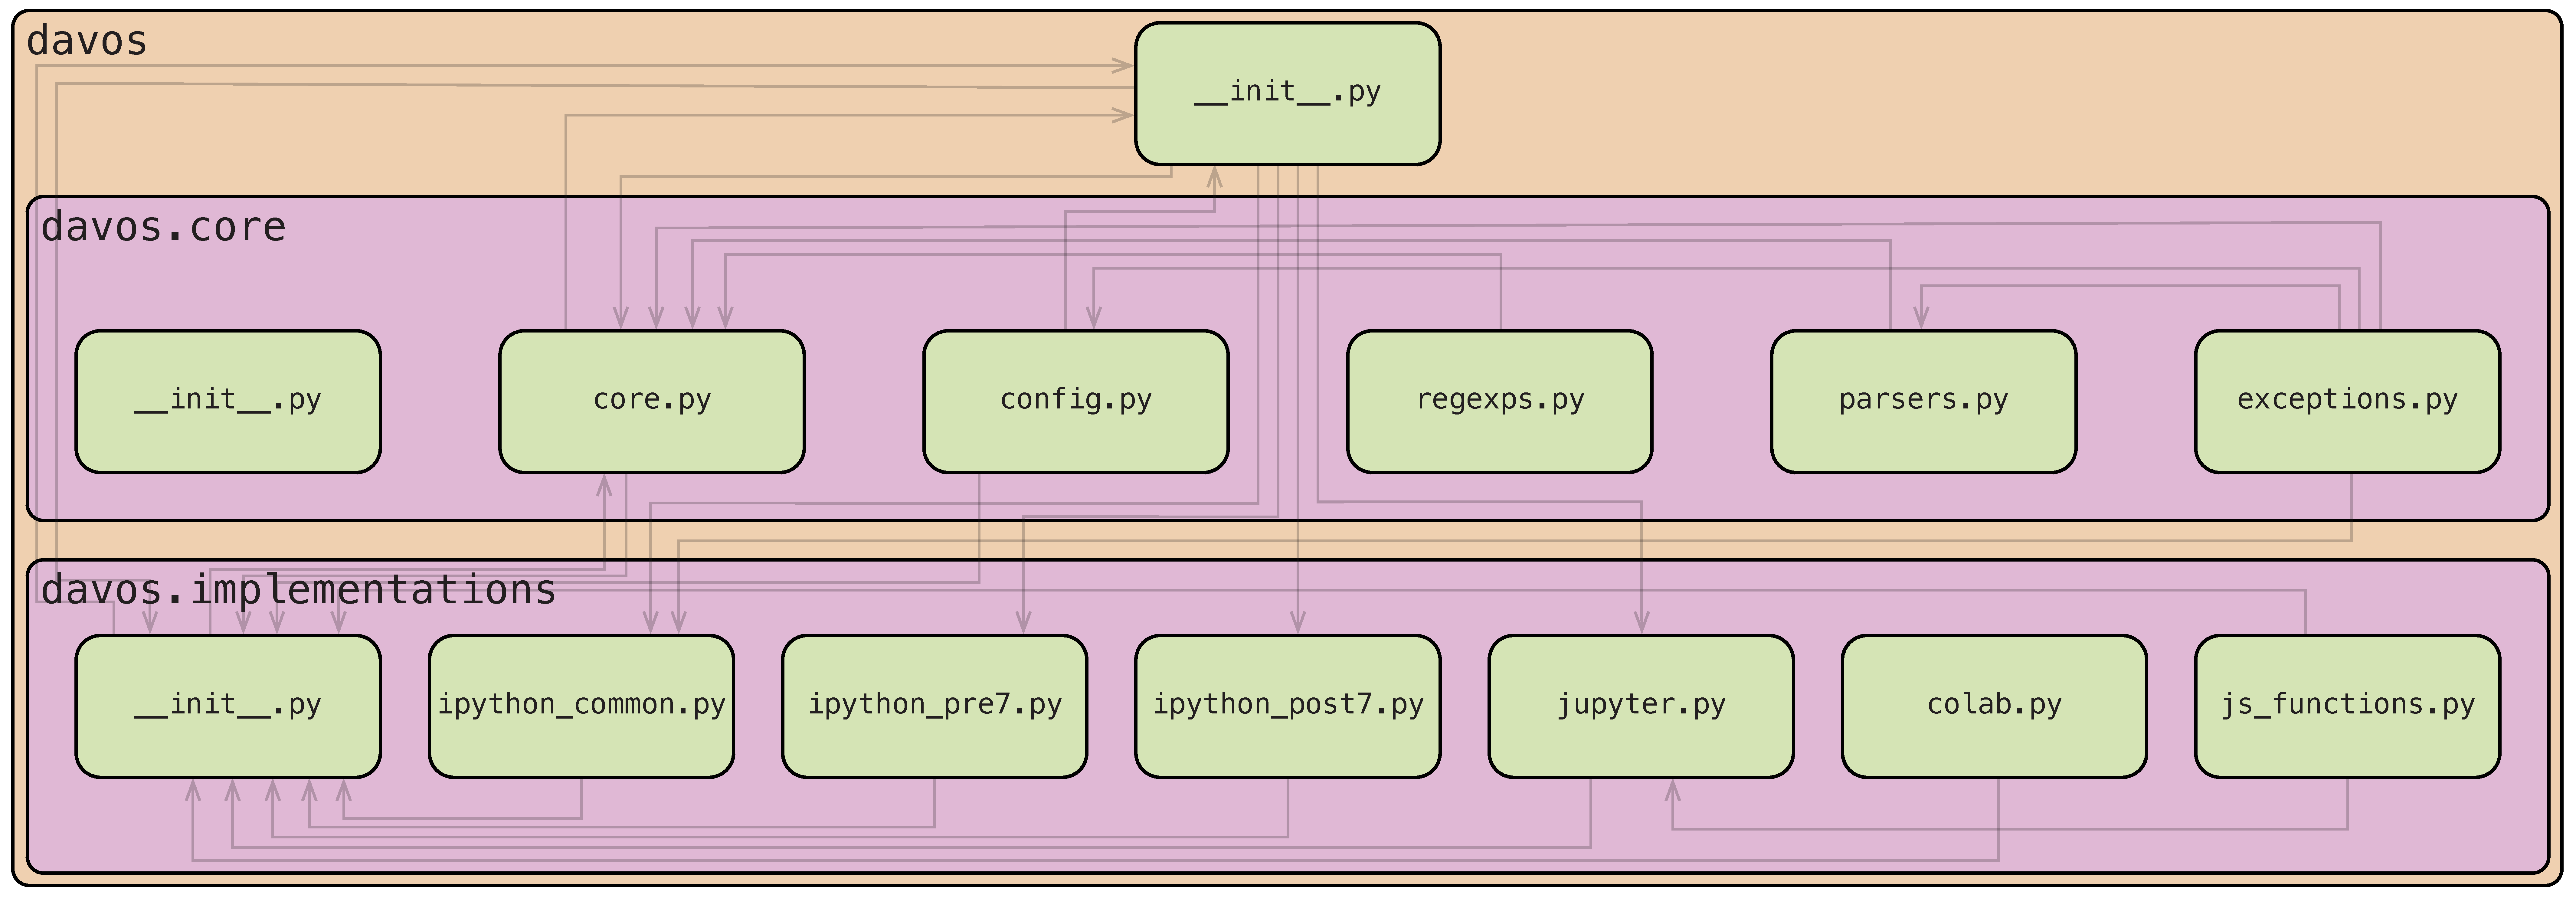
\includegraphics[width=\textwidth]{figs/package_structure}
\caption{\small \textbf{Package structure.} }
\label{fig:package-structure}
\end{figure}

\subsection{Software architecture}
% Give a short overview of the overall software architecture; provide a pictorial component overview or similar (if possible). If necessary provide implementation details.
The \texttt{davos} package consists of two interdependent subpackages (see Fig.~\ref{fig:package-structure}). The first, \texttt{davos.core}, comprises a set of modules that implement\comment{provide?} the bulk of the package's core functionality, including pipelines for installing and validating packages, custom parsers for the \texttt{smuggle} statement (see Section~\ref{subsec:smuggle}) and onion comment (see Section~\ref{subsec:onion}), and a runtime interface for configuring \texttt{davos}'s behavior (see Section~\ref{subsec:config}). However, certain critical\comment{other important} aspects of this functionality require (often substantially) different implementations depending on properties of the notebook environment in which \texttt{davos} is used (e.g., whether the frontend is provided by Jupyter or Google Colaboratory, or which version of IPython~\cite{PereGran07} is used by the notebook kernel). To deal with this, environment-dependent parts of core features and behaviors are isolated and abstracted to ``helper functions'' in the \texttt{davos.implementations} subpackage. This second subpackage defines multiple, interchangeable versions of each helper function, organized into modules by the conditions that trigger their use. At runtime, \texttt{davos} detects various features in the notebook environment and selectively imports a single version of each helper function into the top-level \texttt{davos.implementations} namespace, allowing \texttt{davos.core} modules to access the correct implementations for the current notebook environment in a single, consistent location. An additional benefit of this design pattern is that it allows maintainers or users to easily extend \texttt{davos} to support new, updated, or custom notebook variants by creating a new \texttt{davos.implementations} module with any necessary tweaks to the existing helper functions.

%The package also includes stub files (\texttt{.pyi} files) for each module for use with a static type checker, as well as a custom GitHub Actions-based CI test suite that uses

\comment{
- js_functions.py?
- how parser is registered and deregistered?
- stub files?
- test suite?
- packaged with new PEP \_\_\_ standard (pyproject.toml + setup.cfg; no setup.py)?
}

\subsection{Software functionalities}
% Present the major functionalities of the software.
\subsubsection{The \texttt{smuggle} statement}\label{subsec:smuggle}
Importing \texttt{davos} in an IPython notebook enables an additional Python keyword: ``\texttt{smuggle}'' (see Section~\ref{subsec:implementation} for details on how this works).
The \texttt{smuggle} statement can be used as a drop-in replacement for Python's built-in \texttt{import} statement to load libraries, modules, and other objects into the current namespace.
However, whereas \texttt{import} will fail if the requested package is not installed locally, \texttt{smuggle} statements can handle missing packages on the fly.
If a smuggled package does not exist in the local environment, \texttt{davos} will install it automatically, expose its contents to Python's \texttt{import} machinery, and load it into the namespace for immediate use.

\subsubsection{The onion comment}\label{subsec:onion}
For greater control over the behavior of \texttt{smuggle} statements, \texttt{davos} defines an additional construct called the ``onion comment.'' An onion comment is a special type of inline comment that may be placed on a line containing a \texttt{smuggle} statement to customize how \texttt{davos} searches for the smuggled package locally and, if necessary, downloads and installs it. Onion comments follow a simple format based on the ``type comment'' syntax introduced in PEP 484~\cite{vanREtal14}, and are designed to make managing packages with \texttt{davos} intuitive and familiar. To construct an onion comment, users provide the name of the installer program (e.g., \texttt{pip}) and the same arguments one would use to manually install the package as desired via the command line:
\begin{center}
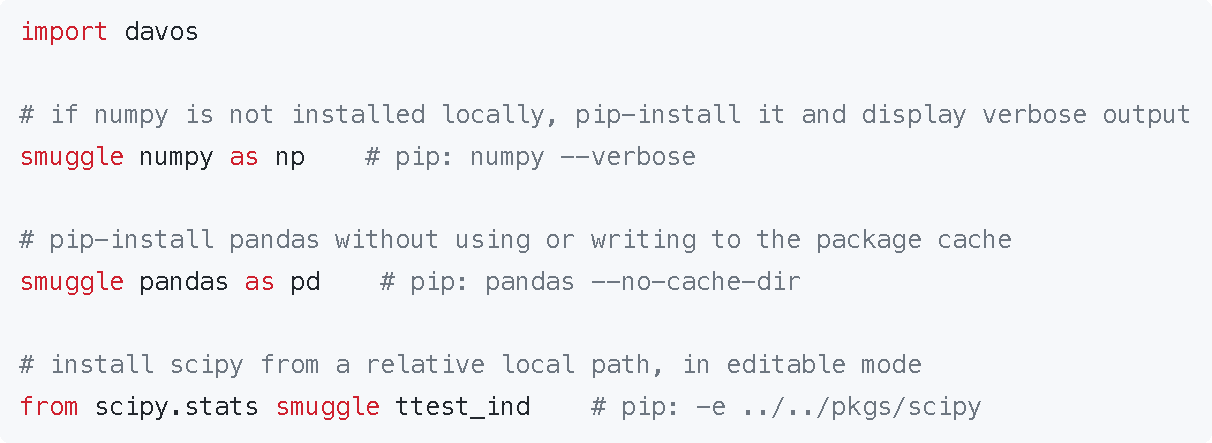
\includegraphics[width=0.9\textwidth]{figs/snippet1}
\end{center}
Occasionally, a package's distribution name (i.e., the name used when installing it) may differ from its top-level module name (i.e., the name used when importing it). In such cases, an onion comment can be used to ensure \texttt{davos} installs the proper distribution if the smuggled package can't be found locally:
%Onion comments are useful in such cases for ensuring \texttt{davos} installs the proper distribution if the smuggled package isn't installed locally:
%Onion comments are useful when smuggling a package whose distribution name (i.e., the name used when installing it) differs from its top-level module name (i.e., the name used when importing it). Onion comments are useful in such cases for
\begin{center}
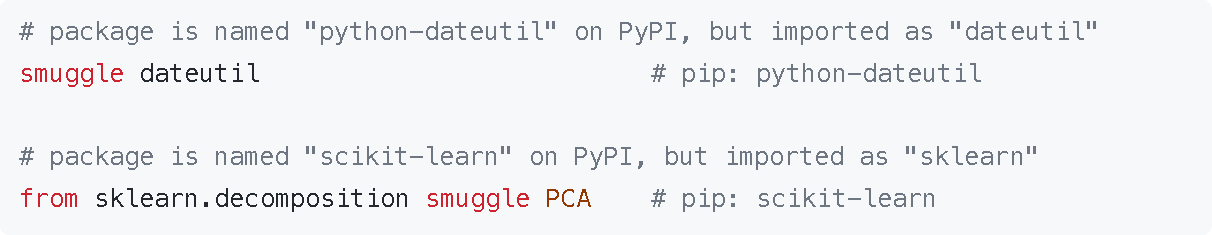
\includegraphics[width=0.9\textwidth]{figs/snippet2}
\end{center}
However, the most powerful use of the onion comment is making \texttt{smuggle} statements \textit{version-sensitive}. If an onion comment includes a version specifier~\cite{CoghStuf13}, \texttt{davos} will ensure that the version of the package loaded into the notebook matches the specific version requested, or satisfies the given version constraints. If the smuggled package exists locally, \texttt{davos} will extract its version info from its metadata and compare it to the specifier provided. If the two are incompatible (or no local installation is found), \texttt{davos} will install and load a suitable version of the package instead:
\begin{center}
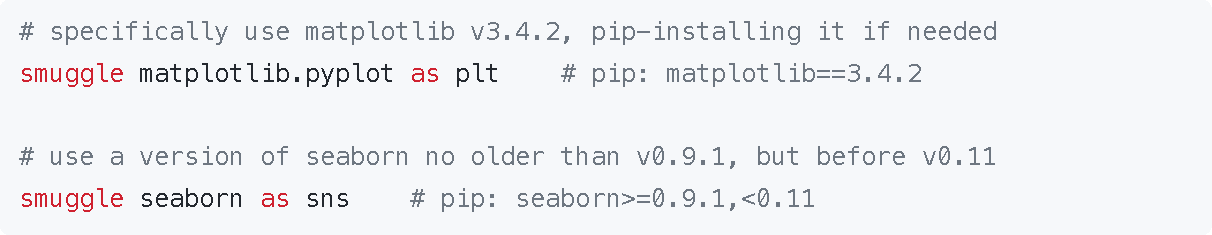
\includegraphics[width=0.9\textwidth]{figs/snippet3}
\end{center}
Onion comments can also be used to smuggle specific VCS references (e.g., Git~\cite{TorvHama05}  branches, commits, tags, etc.):
\begin{center}
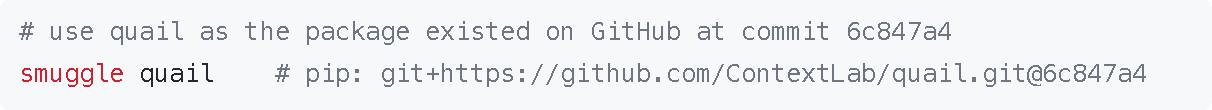
\includegraphics[width=0.9\textwidth]{figs/snippet4}
\end{center}
\texttt{davos} processes onion comments internally before forwarding arguments to the installer program. In addition to preventing onion comments from being used as a vehicle for shell injection attacks, this allows \texttt{davos} to take certain logical actions when particular arguments are passed. For example, the \texttt{-I}/\newline\texttt{--ignore-installed}, \texttt{-U}/\texttt{--upgrade}, and \texttt{--force-reinstall} flags will all cause \texttt{davos} to skip searching for a smuggled package locally before installing a new copy:
\begin{center}
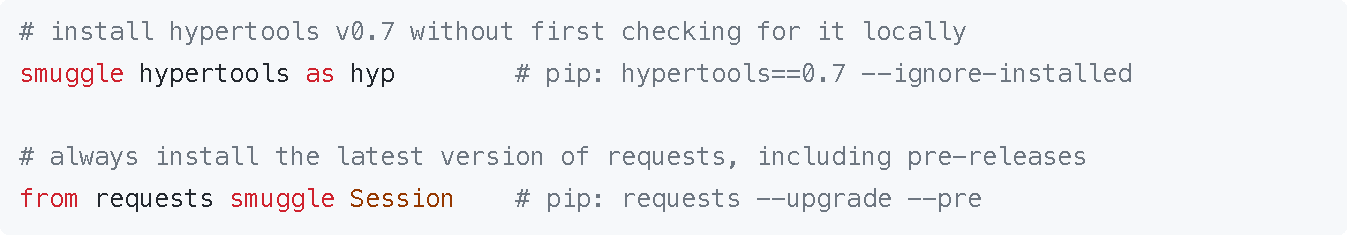
\includegraphics[width=0.9\textwidth]{figs/snippet5}
\end{center}
Similarly, passing \texttt{--no-input} will temporarily enable \texttt{davos}'s non-interactive mode (see Section~\ref{subsec:config}), and installing a smuggled package into \texttt{<dir>} with \texttt{--target <dir>} will cause \texttt{dir} to be prepended to the module search path (\texttt{sys.path}), if necessary, so the package can be imported

\subsubsection{The \texttt{davos} config}\label{subsec:config}
The \texttt{davos} config provides a simple, high-level interface for controlling various aspects of \texttt{davos}'s behavior. After importing \texttt{davos}, the \texttt{davos.config} object (a singleton) exposes a number of configurable options as attributes that can be assigned different values, checked at runtime, and displayed in the notebook cell output (see Fig.~\textcolor{red}{INSERT REF TO ILLUSTRATIVE EXAMPLE FIG} for example usage). These include:
%The \texttt{davos.config} object provides a simple, high-level interface for controlling various aspects of \texttt{davos}'s behavior. After importing \texttt{davos}, the config instance (a singleton) for the current session exposes a number of options that can be set by assigning values to the object's attributes (see Fig.~\textcolor{red}{INSERT REF TO ILLUSTRATIVE EXAMPLE FIG} for example usage). These include:
%The \texttt{davos} config object provides a simple, high-level interface that allows users to view and set various options that affect \texttt{davos}'s behavior. After importing \texttt{davos}, the config instance (a singleton) for the current session is available as \texttt{davos.config}, and its various fields are accessible as attributes (see Fig.~\textcolor{red}{REF TO ILLUSTRATIVE EXAMPLE FIG} for example usage). The config object exposes a mixture of writable and read-only fields. Writable fields include:
\begin{itemize}
\item \texttt{.active}: This option allows users to disable \texttt{davos} functionality (i.e., support for \texttt{smuggle} statements and onion comments) for subsequent notebook cells by setting its value to \texttt{False}. \texttt{davos} can be re-enabled at any time by setting this option to \texttt{True} (the default when \texttt{davos} is first imported). See Section~\ref{subsec:implementation} for additional info.
\item \texttt{.auto\_rerun}: This option controls how \texttt{davos} behaves when attempting to \texttt{smuggle} a new version of a package that was previously imported and cannot be reloaded. This can happen if the package includes extension modules that dynamically link C or C++ objects to the Python interpreter itself, and the code that generates those objects was changed between the old and new versions. If this option is set to \texttt{True}, \texttt{davos} will automatically restart the notebook kernel and rerun all code up to (and including) the current \texttt{smuggle} statement. If \texttt{False} (the deafult), \texttt{davos} will instead issue a warning, pause execution, and prompt the user with buttons to either restart and rerun the notebook, or continue running with the previously imported package version until the next time the kernel is restarted manually. (Note: not configurable in Google Colaboratory).
%\item \texttt{.auto\_rerun}: Some packages (e.g., \texttt{numpy}, \texttt{pandas}) contain extension modules that dynamically link C or C++ objects to the Python interpreter when imported. If \texttt{davos} is used to \texttt{smuggle} a specific version of such a package after a different version of the same package was previously imported
%\item \texttt{.auto\_rerun}: This option controls how \texttt{davos} behaves when attempting to \texttt{smuggle} a new version of a package that was previously imported (at a different version) and cannot be reloaded (i.e., because it contains C-extensions that dynamically generate code). If \texttt{True} (default: \texttt{False}), \texttt{davos} will automatically restart the notebook kernel and rerun all code up to (and including) the current \texttt{smuggle} statement. Otherwise, \texttt{davos} will issue a warning, pause execution, and prompt the user with buttons to either restart and rerun the notebook or continue running with the imported package version. (Note: not configurable in Google Colaboratory).
\item \texttt{.confirm\_install}: If \texttt{True} (default: \texttt{False}), \texttt{davos} will require user confirmation (\texttt{[y]es/[n]o} input) before installing a smuggled package.
\item \texttt{.noninteractive}: Setting this option to \texttt{True} (default: \texttt{False}) enables non-interactive mode, in which all user input and confirmation is disabled. Note that in non-interactive mode, the \texttt{confirm\_install} option is set to \texttt{False}, and if \texttt{auto\_rerun} is \texttt{False}, \texttt{davos} will throw an error if a smuggled package cannot be reloaded, rather than prompting the user.
\item \texttt{.pip\_executable}: This option's value specifies the path to the \texttt{pip} executable used to install smuggled packages. The default is programmatically determined from the Python environment and falls back to \texttt{sys.executable -m pip} if no executable can be found.
\item \texttt{.suppress\_stdout}: If \texttt{True} (default: \texttt{False}), suppress all unnecessary output issued by both \texttt{davos} and the installer program. This can be useful when smuggling packages that need to install many dependencies and/or generate extensive output. If the installer program throws an error, both the stdout and stderr streams will be displayed with the traceback.
\end{itemize}

%\noindent The \texttt{davos.config} object also provides a few informative read-only fields, including:
%\begin{itemize}
%\item \texttt{.environment}: This field's value is a short string describing the notebook environment in which \texttt{davos} is currently running. This is used internally may be one of \texttt{IPython<7.0} (a notebook whose frontend uses the Jupyter JavaScript library and whose backend uses an IPython version older than v7.0), \texttt{IPython>=7.0} (, or \texttt{}
%\end{itemize}
\noindent The top-level \texttt{davos} namespace also defines a handful of convenience functions for setting and checking \texttt{davos}'s active/inactive state (\texttt{davos.activate()}; \texttt{davos.deactivate()}; \texttt{davos.is\_active()}) as well as the \texttt{davos.configure()} function, which allows setting multiple config options at once.

\subsection{Implementation details}\label{subsec:implementation}
Functionally, importing \texttt{davos} appears to make ``\texttt{smuggle}'' a valid Python keyword, similar to standard keywords like ``\texttt{import}'', ``\texttt{def}'', or ``\texttt{return}''. It also appears to fundamentally change how Python treats comments, suddenly allowing them to potentially influence code behavior at runtime if they conform to a particular syntax. However, \texttt{davos} doesn't actually modify the rules of Python's parser or lexical analyzer in order to accomplish this---in fact, modifying the Python grammar isn't possible at runtime, as doing so would require rebuilding the interpreter. Instead, \texttt{davos} leverages the IPython notebook backend to implement the \texttt{smuggle} statement and onion comment via a combination of namespace injections and its own (far simpler) custom parser.

The \texttt{smuggle} keyword can be enabled and disabled at any time by ``activating'' and ``deactivating'' \texttt{davos} (see Section~\ref{subsec:config}, above). When \texttt{davos} is first imported, it is activated automatically. Activating \texttt{davos} triggers two actions: (1) the \texttt{smuggle()} function is injected into the IPython user namespace, and (2) the \texttt{davos} parser is registered as a custom IPython input transformer. IPython preprocesses all executed code as plain text before it is sent to the Python compiler, in order to handle special constructs like \texttt{\%magic} and \texttt{!shell} commands. \texttt{davos} hooks into this process to transform \texttt{smuggle} statements into syntactically valid Python code. The \texttt{davos} parser uses a complex regular expression~\cite{Thom68} to match lines of code containing \texttt{smuggle} statements (and, optionally, onion comments), extract relevant information from their text, and replace them with equivalent calls to the \texttt{smuggle()} function. For example, if a user runs a notebook cell containing
\begin{center}

\includegraphics[width=0.9\textwidth]{figs/snippet6}
\end{center}
the code that is actually executed by the Python interpreter would be
\begin{center}
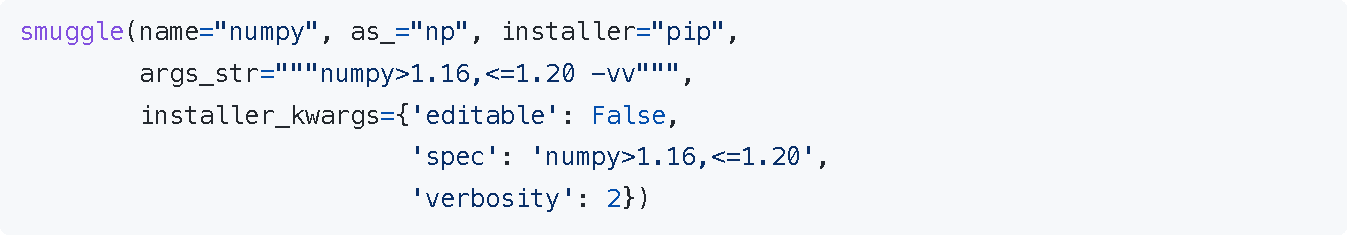
\includegraphics[width=0.9\textwidth]{figs/snippet7}
\end{center}
The call to the \texttt{smuggle()} function then carries out \texttt{davos}'s central logic of determining whether the smuggled package should be installed, doing so if necessary, and subsequently loading it into the namespace. This process is outlined in Figure \ref{fig:flow-chart}. Because the \texttt{smuggle()} function is defined in the notebook namespace, it is also possible (though never necessary) to call it directly. Deactivating \texttt{davos} will delete the name ``\texttt{smuggle}'' from the namespace, unless its value has been overwritten and no longer refers to the \texttt{smuggle()} function. It will also deregister the \texttt{davos} parser from the set of input transformers run when each notebook cell is executed. While the overhead added by the \texttt{davos} parser is minimal, this may be useful, for example, when optimizing or precisely profiling code.

\begin{figure}[tp]
\centering
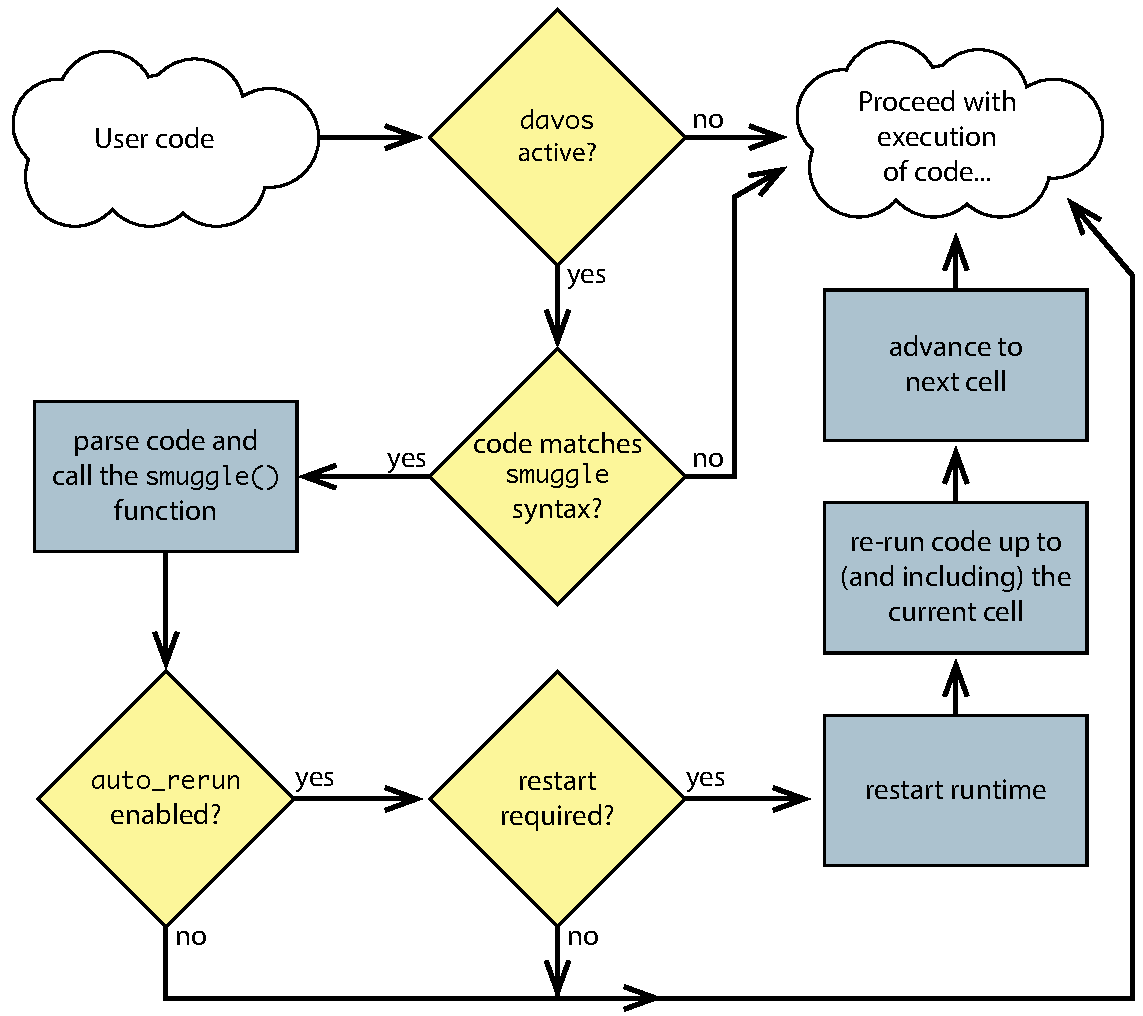
\includegraphics[width=\textwidth]{figs/flow_chart}
\caption{\small \textbf{\texttt{smuggle()} function logic.} }
\label{fig:flow-chart}
\end{figure}

% talk about how exceptions have to inherit from SyntaxError since that's the only thing that can be raised during parsing


% ----------------------------------------------- ILLUSTRATIVE EXAMPLES ------------------------------------------------
\section{Illustrative Examples}
% Provide at least one illustrative example to demonstrate the major functions.

% Optional: you may include one explanatory video that will appear next to your article, in the right hand side panel. (Please upload any video as a single supplementary file with your article. Only one MP4 formatted, with 50MB maximum size, video is possible per article. Recommended video dimensions are 640 x 480 at a maximum of 30 frames/second. Prior to submission please test and validate your .mp4 file at $ http://elsevier-apps.sciverse.com/GadgetVideoPodcastPlayerWeb/verification$. This tool will display your video exactly in the same way as it will appear on ScienceDirect.).


% ------------------------------------------------------- IMPACT -------------------------------------------------------
\section{Impact}

Like virtual environments, containers, and virtual machines, the
\texttt{davos} library (when used in conjunction with Jupyter
notebooks) provides a light\-weight mechanism for sharing code and
ensuring reproducibility across users and computing environments
(Fig.~\ref{fig:code-sharing}). Further, \texttt{davos} enables users
to fully specify (and install, as needed) any project dependencies
within the same notebook. This provides a system whereby executable
code (along with text and media) \textit{and} code for setting up and
configuring the project dependencies, may be combined within a single
notebook file.

We designed \texttt{davos} for use in research applications. For
example, in many settings, \texttt{davos} may be used as a drop-in
replacement for more-difficult-to-set-up virtual environments,
containers, and/or virtual machines. For researchers, this lowers
barriers to both sharing code. By eliminating most of the setup costs
of reconstructing the original researchers' computing environment,
\texttt{davos} also lowers barriers to entry for members of
the scientific community and the public who seek to benefit
from shared code.

Beyond research applications, \texttt{davos} is also useful in
pedagogical settings. For example, in programming courses,
instructors and students may import the \texttt{davos} library into
their notebooks to provide a simple means of ensuring their code will
run on others' machines. When combined with online notebook-based
platforms like Google Colaboratory, \texttt{davos} provides a
convenient way to manage dependencies within a notebook, without
requiring any software (beyond a web browser) to be installed on the
students' or instructors' systems. For the same reasons,
\texttt{davos} also provides an elegant means of sharing ready-to-run
notebook-based demonstrations or tutorials that install their dependencies
automatically.

Since its initial release, \texttt{davos} has found use in a variety
of applications. In addition to managing computing environments
for multiple ongoing research studies, \texttt{davos} is being used by
both students and instructors in programming and methods courses such as
Storytelling with Data~\cite{Mann21d} (an open course on data science,
visualization, and communication) and Laboratory in Psychological
Science~\cite{Mann22} (an open course on experimental and statistical
methods for psychology research) to simplify distributing lessons and
submitting assignments, as well as in online demos such as
\texttt{abstract2paper}~\cite{Mann21e} (an example application of
GPT-Neo~\cite{GaoEtal20, BlacEtal21}) to share ready-to-run code that
installs dependencies automatically.

Our work also has several more subtle ``advanced'' use cases and
potential impacts. Whereas Python's built-in \texttt{import}
statement is agnostic to packages' version information, \texttt{smuggle}
statements (when combined with onion comments) are version-sensitive.
And because onion comments are parsed at runtime, required packages and
their specified versions are installed in a just-in-time manner. Thus, it is possible
in most cases to \texttt{smuggle} a specific package version or revision even if
a different version has already been loaded. This enables more complex uses
that take advantage of multiple versions of a package within a single interpreter
session. This could be useful in cases where specific features are added or
removed from a package across different versions, or in comparing the
performance or functionality of particular features across different versions of
the same package.

A second advanced use case is in providing a proof-of-concept of how
one can add new ``keyword-like'' operators to the Python language by
leveraging notebooks' error-handling mechanisms. This could lead to
exciting new tools that, like \texttt{davos}, extend the Python
language in useful ways within notebook-based environments. We note that
our approach to adding the \texttt{smuggle} keyword to Python when
\texttt{davos} is imported into a notebook-based environment also has
the potential to be exploited for more nefarious purposes. For
example, a malicious user could use a similar approach (e.g., in a
different library) to substantially change a notebook's functionality
by adding new \textit{unexpected} keyword-like objects (e.g., based
around common typos). This could lead to difficult-to-predict changes
in a notebook's behavior once the malicious library was imported.
This highlights an important reason why security-conscious users would
be well-served to only make use of libraries from trusted sources, or
whose code is publicly available for review.

% ---------------------------------------------------- CONCLUSIONS -----------------------------------------------------
\section{Conclusions}
% Set out the conclusion of this original software publication.

The \texttt{davos} library supports reproducible research by providing
a novel lightweight system for sharing notebook-based code. But
perhaps the most exciting uses of the \texttt{davos} library are those
that we have \textit{not} yet considered or imagined. We hope that
the Python community will find \texttt{davos} to provide a convenient
means of managing project dependencies to facilitate code sharing. We
also hope that some of the more advanced applications of our library
might lead to new insights or discoveries.


\section*{Author Contributions}
\textbf{Paxton C. Fitzpatrick}: Conceptualization, Methodology,
Software, Validation, Writing - Original Draft,
Visualization. \textbf{Jeremy R. Manning}: Conceptualization,
Resources, Validation, Writing - Review \& Editing, Supervision, Funding
acquisition.

\section*{Funding}
Our work was supported in part by NSF grant number 2145172 to JRM.
The content is solely the responsibility of the authors and does not necessarily represent the official views of our supporting organizations.


\section*{Declaration of Competing Interest}
We wish to confirm that there are no known conflicts of interest associated with this publication and there has been no significant financial support for this work that could have influenced its outcome.


\section*{Acknowledgements}
We acknowledge useful feedback and discussion from the students of
JRM's \textit{Storytelling with Data} course (Winter, 2022 offering)
who used preliminary versions of our library in several assignments.

%---------------------------------------------------- BIBLIOGRAPHY -----------------------------------------------------
\bibliographystyle{elsarticle-num}
\bibliography{cdl}

\end{document}

